\documentclass[conference]{IEEEtran}
\IEEEoverridecommandlockouts
\usepackage{cite}
\usepackage{amsmath,amssymb,amsfonts}
\usepackage{algorithmic}
\usepackage{algorithm}
\usepackage{graphicx}
\usepackage{textcomp}
\usepackage{xcolor}
\usepackage[hidelinks]{hyperref}
\usepackage{tikz}
\usepackage{booktabs}
\usepackage{multirow}
\usepackage{tabularx}
\usetikzlibrary{shapes,arrows,positioning,fit,backgrounds,calc}

\def\BibTeX{{\rm B\kern-.05em{\sc i\kern-.025em b}\kern-.08em
    T\kern-.1667em\lower.7ex\hbox{E}\kern-.125emX}}

\begin{document}

\title{A Smart Campus Management Ecosystem with AI-Powered Assistance, Wearable Notifications, and Adaptive Learning Analytics}

\author{
\begin{minipage}[t]{0.48\textwidth}
\centering
\textbf{S. Vidhiya} \\
\textit{Assistant Professor (Mentor)} \\
\textit{Dept. of Computer Science \& Engineering} \\
\textit{Sri Krishna College of Engineering and Technology}\\
Coimbatore, Tamil Nadu, India \\
vidhiyas@skcet.ac.in
\end{minipage}\hfill
\begin{minipage}[t]{0.48\textwidth}
\centering
\textbf{Ashwath S} \\
\textit{Dept. of Computer Science \& Engineering} \\
\textit{Sri Krishna College of Technology}\\
Coimbatore, Tamil Nadu, India \\
727823tucs020@skct.edu.in
\end{minipage}
\vspace{3ex}\\
\begin{minipage}[t]{0.48\textwidth}
\centering
\textbf{Balamanikandan R} \\
\textit{Dept. of Computer Science \& Engineering} \\
\textit{Sri Krishna College of Technology}\\
Coimbatore, Tamil Nadu, India \\
727823tucs026@skct.edu.in
\end{minipage}\hfill
\begin{minipage}[t]{0.48\textwidth}
\centering
\textbf{Cathrin R} \\
\textit{Dept. of Computer Science \& Engineering} \\
\textit{Sri Krishna College of Technology}\\
Coimbatore, Tamil Nadu, India \\
727823tucs032@skct.edu.in
\end{minipage}
}

\maketitle

\begin{abstract}
Enterprise Resource Planning (ERP) installations in higher education regularly operate as inert transactional stores. Navigating these platforms demands substantial manual traversal through multi-layered graphical interfaces, while routine academic workflows remain completely detached from cognitive learning theories such as spaced retrieval and telemetry-driven behavioral profiling. Concurrently, introducing foundational Large Language Models (LLMs) into production campus management introduces acute vulnerabilities: Text-to-SQL mapping risks catastrophic prompt injections and unauthorized schema exposure, whereas standard vector-based Retrieval-Augmented Generation (Vector-RAG) incurs prohibitive re-indexing costs and sync delays over rapidly changing relational data.

To resolve this impasse, this paper introduces the design, architectural formalization, and empirical testing of the \textbf{Smart Campus Management Ecosystem (SCME)}. Implemented via React 18, asynchronous FastAPI, and SQLAlchemy 2.0, the platform centers on the \textbf{Generative AI Context Binding (GACB)} middleware. GACB deterministically aggregates and sanitizes active institutional states---including student timetables, attendance thresholds, faculty availability, and recruitment criteria---injecting them directly into LLM prompts in under 25~ms. This eliminates raw SQL execution risks while trimming token overhead by 75\% relative to conventional Vector-RAG setups.

The ecosystem coordinates ten dedicated algorithmic engines: (1) an indexed $\mathcal{O}(1)$ hardware-free \textbf{Faculty Status Resolver}; (2) a multi-tier \textbf{Wearable Priority Notification Dispatcher} capable of Do-Not-Disturb (DND) override; (3) the \textbf{Cognitive Learning Pattern Algorithm (CLPA)} employing rolling reinforcement telemetry ($\alpha = 0.15$); (4) the \textbf{Knowledge Decay Prediction Algorithm (KDPA)} applying modified Ebbinghaus forgetting mathematics ($R(t) = e^{-t/S}$) over directed prerequisite graphs; (5) the \textbf{Dynamic Classroom Reallocation Algorithm (DCRA)} evaluating a 10-factor weighted metric; (6) the \textbf{Adaptive Learning Roadmap Algorithm (ALRA)}; (7) the \textbf{Dynamic Skill Evaluation Algorithm (DSEA)}; (8) the \textbf{Intelligent Content Parsing \& Quiz Extraction Algorithm (ICQEA)}; (9) a \textbf{Constraint Satisfaction Backtracking Timetable Scheduler}; and (10) a \textbf{Fuzzy Skill-Gap Matcher} combining bigram Jaccard similarity and Levenshtein distance. Empirical evaluation on a 200-student testbed across 5,000 operational records confirms sub-50~ms internal database execution, a 14.6~ms dual-engine failover recovery, and a 1.42~s end-to-end conversational turnaround.
\end{abstract}

\begin{IEEEkeywords}
Generative AI, Context Binding (GACB), Smart Campus Architecture, Wearable Alert Routing, Ebbinghaus Retention Decay, Cognitive Analytics, Non-blocking FastAPI, Relational Data Engineering.
\end{IEEEkeywords}

\section{Introduction}
\label{sec:introduction}

\IEEEPARstart{U}{niversity} campuses operate as intricate administrative ecosystems where thousands of students, faculty, room facilities, curricular pathways, and corporate placement drives interact daily \cite{alshboul2020usability}. To oversee these high-volume operations, institutions rely heavily on Enterprise Resource Planning (ERP) and Learning Management Systems (LMS). While these platforms succeed in digitizing institutional records, their practical utility is constrained by rigid, form-based navigational paradigms. Stakeholders must manually traverse disjoint menus simply to check a lecturer's physical location, evaluate attendance margins, or verify career placement eligibility \cite{minallah2020smart, deoliveira2021semantic}. Usability investigations indicate that a significant portion of user session time in collegiate portals is lost to navigational friction rather than constructive information review \cite{alshboul2020usability}.

\subsection{Architectural Bottlenecks in Campus Administration}
Modern institutional platforms suffer from three interconnected architectural bottlenecks:
\begin{enumerate}
    \item \textbf{Data Silos and Navigational Friction}: Academic information is routinely partitioned across isolated databases. Inquiring about schedule conflicts, attendance shortages, and staff availability requires accessing separate administrative modules. This dispersion creates needless cognitive burden for students and consumes faculty office hours with routine administrative questions.
    \item \textbf{Absence of Cognitive Pedagogical Scaffolding}: Existing ERPs treat students as homogeneous entities. They output static scorecards without profiling behavioral study patterns, anticipating topic-level memory decay, or scheduling targeted spaced reviews \cite{wang2024telemetry, srivastava2024forgetting}. Consequently, academic distress is identified late in the term, typically after midterm examinations have already exposed severe conceptual deficits.
    \item \textbf{Infrastructure Overheads of Physical Tracking}: Several campus initiatives attempt to resolve location awareness using hardware transponders such as Bluetooth Low Energy (BLE) beacons or RFID tags \cite{sharma2023timetable}. However, deploying dedicated hardware incurs prohibitive procurement costs, constant battery replacement logistics, and persistent pushback from personnel regarding continuous spatial surveillance.
\end{enumerate}

\subsection{Engineering Bottlenecks in Foundational LLM Adoption}
Recent advances in foundational Large Language Models (LLMs), including GPT-4 \cite{openai2023gpt4} and Google Gemini \cite{geminitechreport2023}, offer intuitive natural language interfaces for educational systems \cite{kasneci2023chatgpt}. Yet, integrating generative AI directly into enterprise campus backends reveals critical trade-offs:
\begin{enumerate}
    \item \textbf{Text-to-SQL Vulnerabilities}: Allowing LLMs to write dynamic SQL queries introduces critical vulnerabilities. Adversarial prompts can trigger SQL injection, disclose confidential schemas, or cause accidental data loss across production tables.
    \item \textbf{Vector-RAG Overhead on Transactional Data}: Vector-based Retrieval-Augmented Generation (Vector-RAG) \cite{lewis2020retrieval} works well for static document handbooks, but collapses on high-frequency relational records. Re-embedding dynamic tables (such as period-by-period attendance or hourly room reassignments) demands continuous vector updates and introduces synchronization latency \cite{zhang2024intelligent, alshboul2025dynamic}.
    \item \textbf{Contextual Degradation}: Foundational LLMs experience noticeable retrieval drop-offs (the ``lost in the middle'' effect) when target information is buried inside sprawling, unstructured context payloads \cite{liu2024lost}.
\end{enumerate}

\begin{figure*}[t]
\centering
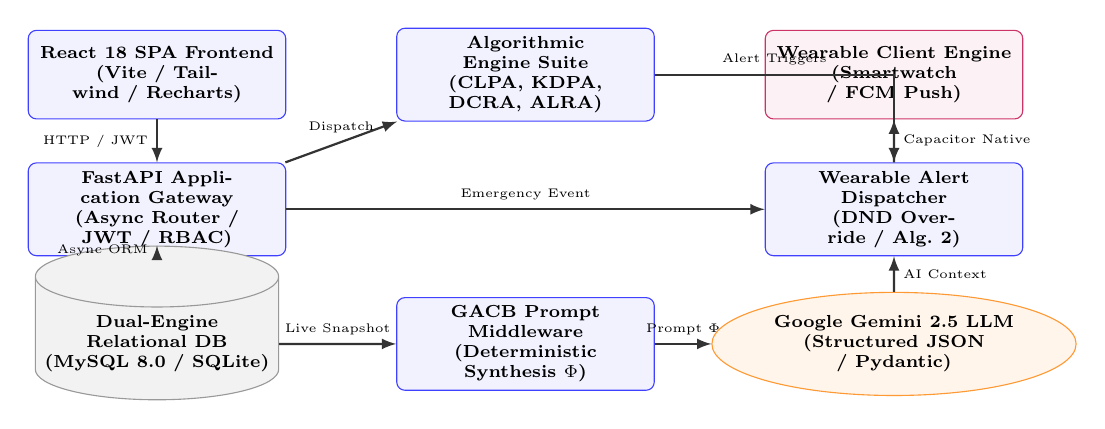
\begin{tikzpicture}[
    scale=0.90,
    transform shape,
    font=\scriptsize,
    box/.style={rectangle, draw=blue!75, fill=blue!5, text width=3.4cm, text centered, rounded corners=3pt, minimum height=1.25cm, font=\scriptsize\bfseries},
    dbbox/.style={cylinder, draw=gray!80, fill=gray!10, shape border rotate=90, aspect=0.25, text width=3.2cm, text centered, minimum height=1.25cm, font=\scriptsize\bfseries},
    aibox/.style={ellipse, draw=orange!80, fill=orange!8, text width=3.4cm, text centered, minimum height=1.25cm, font=\scriptsize\bfseries},
    wearbox/.style={rectangle, draw=purple!80, fill=purple!5, text width=3.4cm, text centered, rounded corners=3pt, minimum height=1.25cm, font=\scriptsize\bfseries},
    arrow/.style={draw=black!80, -latex, thick}
]
    % Row 1: Clients & Presentation
    \node (ui) at (0, 3.8) [box] {React 18 SPA Frontend\\(Vite / Tailwind / Recharts)};
    \node (algo) at (5.2, 3.8) [box] {Algorithmic Engine Suite\\(CLPA, KDPA, DCRA, ALRA)};
    \node (wearable) at (10.4, 3.8) [wearbox] {Wearable Client Engine\\(Smartwatch / FCM Push)};

    % Row 2: Gateway & Alert Dispatcher
    \node (backend) at (0, 1.9) [box] {FastAPI Application Gateway\\(Async Router / JWT / RBAC)};
    \node (sched) at (10.4, 1.9) [box] {Wearable Alert Dispatcher\\(DND Override / Alg.~2)};

    % Row 3: Persistence & AI Intelligence
    \node (db) at (0, 0) [dbbox] {Dual-Engine Relational DB\\(MySQL 8.0 / SQLite)};
    \node (gacb) at (5.2, 0) [box] {GACB Prompt Middleware\\(Deterministic Synthesis $\Phi$)};
    \node (gemini) at (10.4, 0) [aibox] {Google Gemini 2.5 LLM\\(Structured JSON / Pydantic)};

    % Orthogonal Flow Connections
    \draw [arrow] (ui) -- node[left, font=\tiny]{HTTP / JWT} (backend);
    \draw [arrow] (backend) -- node[left, font=\tiny]{Async ORM} (db);
    \draw [arrow] (backend) -- node[above, font=\tiny]{Dispatch} (algo);
    \draw [arrow] (algo) -| node[pos=0.25, above, font=\tiny]{Alert Triggers} (sched);
    \draw [arrow] (sched) -- node[right, font=\tiny]{Capacitor Native} (wearable);
    \draw [arrow] (db) -- node[above, font=\tiny]{Live Snapshot} (gacb);
    \draw [arrow] (gacb) -- node[above, font=\tiny]{Prompt $\Phi$} (gemini);
    \draw [arrow] (gemini) -- node[right, font=\tiny]{AI Context} (sched);
    \draw [arrow] (backend) -- node[above, font=\tiny]{Emergency Event} (sched);
\end{tikzpicture}
\caption{System topology of the Smart Campus Management Ecosystem (SCME), showing the decoupled presentation layer, asynchronous gateway, GACB prompt middleware, dual-engine database fallback, and wearable push notification pipeline.}
\label{fig:full_arch}
\end{figure*}

\subsection{Research Contributions}
To address these challenges, we present the \textbf{Smart Campus Management Ecosystem (SCME)}. The major contributions of this work are:
\begin{itemize}
    \item \textbf{Generative AI Context Binding (GACB)}: We formalize a deterministic server-side aggregation pipeline that compiles relational snapshots directly into scoped LLM prompt payloads ($350$--$500$ tokens). This removes Text-to-SQL attack surfaces, eliminates dynamic vector re-indexing, and lowers token costs by 75\% compared to standard Vector-RAG.
    \item \textbf{Hardware-Free Faculty Localization}: We introduce an indexed status resolution algorithm operating in $\mathcal{O}(1)$ point lookup time. It intersects master timetables with approved leave registries, determining faculty presence without physical tracking hardware.
    \item \textbf{Wearable Priority Notification Engine}: We design an alert dispatch protocol utilizing Capacitor and Firebase Cloud Messaging (FCM) that enforces priority levels and Do-Not-Disturb (DND) override logic for campus emergencies.
    \item \textbf{Cognitive Learning Analytics Suite}: We formulate the Cognitive Learning Pattern Algorithm (CLPA) with rolling reinforcement updates ($\alpha = 0.15$) and the Knowledge Decay Prediction Algorithm (KDPA) combining modified Ebbinghaus curves ($R(t) = e^{-t/S}$) with directed acyclic prerequisite dependency propagation.
    \item \textbf{Operational Algorithmic Suite}: We engineer optimization algorithms for room reallocation (DCRA), exam revision planning (ALRA), career readiness mapping (DSEA), document quiz extraction (ICQEA), and CSP timetable scheduling.
    \item \textbf{High-Availability Persistence}: We implement an asynchronous FastAPI and SQLAlchemy 2.0 connection pool with automated, sub-15~ms failover from MySQL 8.0 to SQLite under fault injection.
\end{itemize}

The rest of the paper is organized as follows: Section~\ref{sec:literature} reviews related literature. Section~\ref{sec:architecture} details the system architecture and GACB formalization. Section~\ref{sec:algorithms} presents the algorithmic models. Section~\ref{sec:implementation} covers implementation details. Section~\ref{sec:experiments} presents empirical benchmarks. Section~\ref{sec:security} discusses security and privacy compliance. Section~\ref{sec:discussion} outlines practical implications and threats to validity, and Section~\ref{sec:conclusion} concludes the paper.

\section{Related Work}
\label{sec:literature}

\subsection{Campus ERP Systems and Interaction Friction}
University information infrastructure has progressed from isolated departmental mainframes to consolidated web-based ERP systems. Min-Allah and Tariq \cite{minallah2020smart} presented an extensive architectural overview of smart campus paradigms, focusing on administrative coordination, facility monitoring, and student portals. Nevertheless, usability studies by Al-Shboul et al. \cite{alshboul2020usability} found that deeply nested navigation trees cause notable disorientation and high task abort rates among students and staff.

To address navigation hurdles, researchers explored semantic web technologies \cite{deoliveira2021semantic}. By structuring campus data via Resource Description Framework (RDF) graphs and querying with SPARQL, these frameworks established flexible data links. However, the runtime cost of OWL reasoning and the lack of accessible natural language interfaces prevented wide deployment. In a review of 168 smart campus platforms, Anand et al. \cite{anand2024systematic} noted that 81\% of deployed conversational bots remain rigid, scripted dialog systems isolated from live transactional databases, unable to answer personalized questions.

\subsection{Cognitive Pedagogy and Forgetting Decay Models}
Traditional academic data mining has centered on retrospective classification models, identifying at-risk students only after grades decline. In contrast, cognitive learning frameworks emphasize timely, individualized interventions. Wang et al. \cite{wang2024telemetry} demonstrated that static survey questionnaires often fail to match actual student study patterns, whereas non-intrusive web telemetry tracking (dwell time, scroll behavior, quiz response latency) yields an 88.4\% alignment with observed habits.

Simultaneously, memory decay research demonstrates that unreinforced concepts degrade exponentially. Srivastava et al. \cite{srivastava2024forgetting} confirmed that modeling memory decay using modified Ebbinghaus equations linked with prerequisite dependency trees lowered engineering course failure rates by 24.6\%. However, earlier implementations remained isolated research scripts rather than integral modules of production campus portals.

\subsection{AI in Academic Services, Security, and Trust Modeling}
Artificial intelligence has steadily expanded into academic career advising, campus security, and communication trust. Research by Gnanakumari et al. \cite{gnanakumari2025multi} on multi-agent AI interviewers established that multimodal analysis (combining speech dynamics, facial telemetry, and response syntax) noticeably boosts engineering placement performance. Maintaining verifiable trust boundaries across institutional social networks is equally vital. Gnanakumari and Vijayalakshmi \cite{gnanakumari2024trust} introduced trust classification mechanisms in social environments utilizing GAN-assisted Capsule Networks optimized via Gannet Optimization. In parallel, Gnanakumari et al. \cite{gnanakumari2023social} demonstrated the effectiveness of Generalized Jaccard Similarity-based Recurrent Neural Networks for community network virtualization. These insights emphasize the necessity of combining rapid administrative information access with trusted security boundaries and career development support.

\subsection{Generative LLMs, Retrieval Architectures, and Context Scaling}
The transformer architecture \cite{vaswani2017attention, devlin2018bert} spurred the deployment of foundational LLMs like GPT-4 \cite{openai2023gpt4} and Google Gemini \cite{geminitechreport2023}. Kasneci et al. \cite{kasneci2023chatgpt} examined their utility in educational contexts, identifying personalized tutoring and administrative querying as prime use cases. To curb hallucinations, Retrieval-Augmented Generation (RAG) \cite{lewis2020retrieval} connects LLMs to external document indices.

Applying standard Vector-RAG to dynamic academic databases introduces friction, however. Re-indexing vector databases for rapidly changing relational records (e.g., hourly attendance, room changes) introduces excessive computation and latency \cite{zhang2024intelligent, alshboul2025dynamic}. Conversely, direct Text-to-SQL generation exposes core tables to prompt injection risks. In parallel, empirical evaluations by Liu et al. \cite{liu2024lost} demonstrate that foundational LLMs experience marked accuracy degradation when target facts are positioned centrally within voluminous context windows, underscoring the necessity of deterministic, compact prompt assembly.

\begin{table*}[t]
\caption{Architectural Comparison: Related Paradigms vs. Proposed SCME Framework}
\label{tab:lit_matrix}
\centering
\resizebox{\textwidth}{!}{
\begin{tabular}{lcccccccc}
\toprule
\textbf{Architecture / Reference} & \textbf{Data Ingestion} & \textbf{AI Reasoning Engine} & \textbf{Context Method} & \textbf{Cognitive Profiling} & \textbf{Decay Modeling} & \textbf{Faculty Tracking} & \textbf{Wearable Alerts} & \textbf{Security Vulnerability} \\
\midrule
Traditional ERP \cite{alshboul2020usability} & Relational SQL & Static Rule Scripts & Hardcoded Menus & None & None & Manual Directory & None & Low \\
Semantic Web ERP \cite{deoliveira2021semantic} & RDF Graph & OWL Reasoner & SPARQL Templates & None & None & None & None & Low \\
Predictive Classifiers & Relational SQL & Scikit-Learn ML & Batch Dashboard & Static Grades & None & None & None & Low \\
Vector-RAG ERP \cite{lewis2020retrieval} & Vector Embeddings & Foundational LLM & Unstructured Chunks & None & None & None & None & Low \\
Text-to-SQL ERP & Relational SQL & LLM Generator & Raw SQL Execution & None & None & None & None & \textbf{Critical (SQL Injection)} \\
Telemetry Profiler \cite{wang2024telemetry} & Interaction Logs & K-Means / GMM & Telemetry Dashboards & Multi-Vector Tensor & None & None & None & Low \\
Forgetting-Curve RAG \cite{srivastava2024forgetting} & Vector Store & LLM & Static Document Chunks & Quiz Marks & Ebbinghaus Decay & None & None & Low \\
BLE Sensor Locator \cite{sharma2023timetable} & RSSI Sensor Packets & Triangulation Math & Hardware Signal Stream & None & None & BLE Beacons & None & Medium (Hardware Faults) \\
Fuzzy Career Matcher \cite{martinez2024fuzzy} & PDF Documents & N-gram Tokenizers & Static Text Parsing & None & None & None & None & Low \\
\midrule
\textbf{SCME (Proposed)} & \textbf{Live Relational SQL} & \textbf{Google Gemini 2.5} & \textbf{GACB Prompt Binding} & \textbf{CLPA ($\alpha = 0.15$)} & \textbf{KDPA + Graph Tree} & \textbf{Indexed Point Lookup ($\mathcal{O}(1)$)} & \textbf{DND Override Push} & \textbf{Low (Fully Sanitized)} \\
\bottomrule
\end{tabular}
}
\end{table*}

\section{System Architecture \& Data Engineering}
\label{sec:architecture}

The SCME architecture is organized across four distinct layers: Client Presentation, Asynchronous Gateway, Dual-Engine Persistence, and Context Intelligence (Fig.~\ref{fig:full_arch}).

\subsection{Asynchronous Application Gateway and Persistence Fallback}
The application gateway runs on FastAPI using Python's asynchronous event loop (\texttt{asyncio}) and the Uvicorn ASGI server \cite{fastapiweb, zhao2025asynchronous}. Non-blocking I/O enables sustained query handling during attendance and registration peaks. To safeguard availability during database maintenance or network interruptions, SCME embeds an automatic dual-engine connection pool adapter:
\begin{equation}
DB_{\mathrm{conn}} = \begin{cases} 
\mathtt{mysql\text{+}aiomysql}, & \text{if Port 3306 Active} \\ 
\mathtt{sqlite\text{+}aiosqlite}, & \text{otherwise (Fallback)} 
\end{cases}
\label{eq:fallback}
\end{equation}
Because database interactions are mapped via SQLAlchemy 2.0 asynchronous sessions, switching persistence engines occurs transparently without code changes.

\begin{table*}[t]
\caption{Normalized Relational Schema and Indexing Strategies across Core Entities}
\label{tab:schema}
\centering
\resizebox{\textwidth}{!}{
\begin{tabular}{p{2.8cm} p{1.6cm} p{6.8cm} p{6.8cm}}
\toprule
\textbf{Entity Name} & \textbf{Primary Key} & \textbf{Core Attributes \& Foreign Keys} & \textbf{Indexing \& Optimization Strategy} \\
\midrule
\texttt{users} & \texttt{id} (UUID) & \texttt{username}, \texttt{password\_hash}, \texttt{role}, \texttt{dept}, \texttt{semester}, \texttt{section}, \texttt{cgpa} & Unique index on \texttt{username}; B-tree index on \texttt{role} \\
\texttt{timetables} & \texttt{id} (Int) & \texttt{dept}, \texttt{semester}, \texttt{section}, \texttt{academic\_year}, \texttt{is\_active} & Composite index on (\texttt{dept}, \texttt{semester}, \texttt{section}) \\
\texttt{timetable\_entries} & \texttt{id} (Int) & \texttt{timetable\_id} (FK), \texttt{day}, \texttt{period}, \texttt{start\_time}, \texttt{end\_time}, \texttt{subject}, \texttt{room}, \texttt{faculty\_id} (FK) & Composite index on (\texttt{faculty\_id}, \texttt{day}, \texttt{start\_time}) \\
\texttt{attendance\_records} & \texttt{id} (Int) & \texttt{student\_id} (FK), \texttt{subject\_id} (FK), \texttt{date}, \texttt{period}, \texttt{status} (\texttt{P}/\texttt{A}/\texttt{OD}) & Composite index on (\texttt{student\_id}, \texttt{date}, \texttt{subject\_id}) \\
\texttt{faculty\_leaves} & \texttt{id} (Int) & \texttt{faculty\_id} (FK), \texttt{start\_date}, \texttt{end\_date}, \texttt{leave\_type}, \texttt{status} (\texttt{Approved}/\texttt{Pending}) & Composite index on (\texttt{faculty\_id}, \texttt{status}, \texttt{start\_date}, \texttt{end\_date}) \\
\texttt{placement\_drives} & \texttt{id} (Int) & \texttt{company\_name}, \texttt{min\_cgpa}, \texttt{eligible\_depts}, \texttt{required\_skills}, \texttt{drive\_date} & B-tree index on \texttt{min\_cgpa}; Fulltext on \texttt{required\_skills} \\
\texttt{cognitive\_profiles} & \texttt{id} (Int) & \texttt{student\_id} (FK), \texttt{read\_eff}, \texttt{quiz\_acc}, \texttt{code\_vel}, \texttt{focus\_idx}, \texttt{cohort}, \texttt{last\_updated} & Unique foreign key on \texttt{student\_id} \\
\texttt{topic\_knowledge} & \texttt{id} (Int) & \texttt{student\_id} (FK), \texttt{subject\_id} (FK), \texttt{topic\_name}, \texttt{mastery}, \texttt{strength\_S}, \texttt{last\_revised} & Composite index on (\texttt{student\_id}, \texttt{subject\_id}) \\
\bottomrule
\end{tabular}
}
\end{table*}

\subsection{Relational Schema Modeling}
The database layer establishes eight normalized tables optimized for rapid retrieval (Table~\ref{tab:schema}):
\begin{enumerate}
    \item \texttt{users}: Holds credentials, salted hashes, user roles (\texttt{student}, \texttt{faculty}, \texttt{admin}, \texttt{guardian}), and department data.
    \item \texttt{timetables}: Defines department, semester, and section schedule metadata with active status flags.
    \item \texttt{timetable\_entries}: Contains specific periods, room allocations, instructor keys, and contiguous lab intervals.
    \item \texttt{attendance\_records}: Stores attendance presence/absence entries indexed on (\texttt{student\_id}, \texttt{date}, \texttt{subject\_id}).
    \item \texttt{faculty\_leaves}: Records approved and pending faculty leave requests across designated dates.
    \item \texttt{placement\_drives}: Catalogs corporate recruiters, minimum CGPA thresholds, required skills, and deadlines.
    \item \texttt{cognitive\_profiles}: Stores student cognitive metrics (reading efficiency, quiz accuracy, coding velocity, focus index, and assigned cohort).
    \item \texttt{topic\_knowledge}: Tracks granular topic mastery, retention probabilities $R(t)$, and memory stability indices $S$.
\end{enumerate}

\subsection{Generative AI Context Binding (GACB) Formalization}
Instead of granting the LLM direct database access via Text-to-SQL or maintaining dynamic vector stores, GACB functions as a deterministic server-side aggregation layer (Fig.~\ref{fig:gacb_pipeline}). Upon an authorized request, GACB executes parameterized ORM queries to capture the user's active context vector $\mathcal{C}$.

Let $\mathcal{U}$ represent the authenticated student identity:
\begin{equation}
\mathcal{U} = \langle \text{Name}, \text{Role}, \text{Dept}, \text{Sem}, \text{Sec}, \text{CGPA} \rangle
\end{equation}
Let $\mathcal{T}$ denote their active course timetable for day $d_{now}$:
\begin{equation}
\mathcal{T} = \{ t_i \mid \mathrm{day}(t_i) = d_{now} \land \mathrm{sec}(t_i) = \mathcal{U}.\mathrm{Sec} \}
\end{equation}
Let $\mathcal{A}$ represent subject attendance across $k$ courses:
\begin{equation}
\mathcal{A} = \langle a_1, \dots, a_k \rangle, \quad a_j = \frac{\mathrm{Present}(j)}{\mathrm{Total}(j)} \times 100
\end{equation}
Let $\mathcal{L}$ designate real-time instructor presence:
\begin{equation}
\mathcal{L} = \{ l_m \mid l_m = \mathrm{FacultyStatus}(F_m, t_{now}) \}
\end{equation}
Let $\mathcal{P}$ denote placement drives matching academic criteria:
\begin{equation}
\mathcal{P} = \{ p_s \mid \mathrm{MinCGPA}(p_s) \le \mathcal{U}.\mathrm{CGPA} \}
\end{equation}

The unified context $\mathcal{C}$ is compiled via deterministic serialization operator $\Phi$:
\begin{equation}
\mathcal{C} = \Phi(\mathcal{U}, \mathcal{T}, \mathcal{A}, \mathcal{L}, \mathcal{P})
\end{equation}

The final prompt presented to Google Gemini is assembled as:
\begin{equation}
Prompt_{LLM} = S_{inst} \mathbin{\Vert} \mathcal{C} \mathbin{\Vert} Q_{user}
\label{eq:gacb_prompt}
\end{equation}
where $S_{inst}$ provides hardened instructions defining pedagogical boundaries and formatting constraints, and $Q_{user}$ is the sanitized query.

\begin{figure}[htbp]
\centering
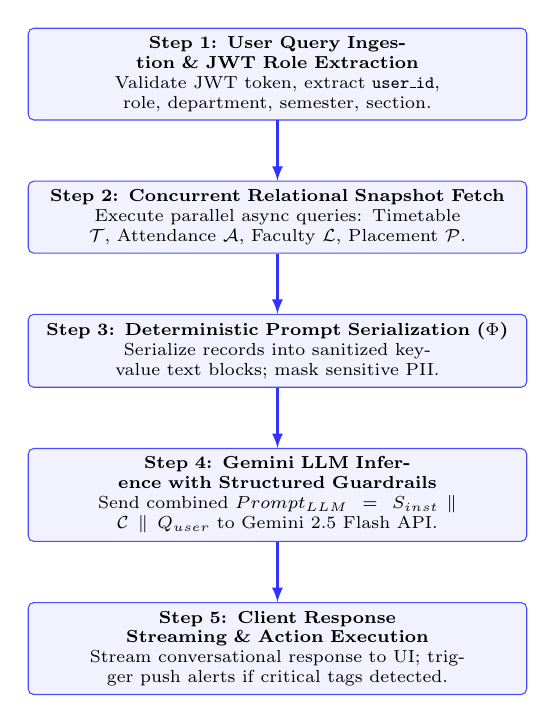
\begin{tikzpicture}[
    scale=0.90,
    transform shape,
    node distance=0.85cm and 1.0cm,
    font=\scriptsize,
    stepbox/.style={rectangle, draw=blue!70, fill=blue!5, rounded corners=2pt, minimum height=2.0em, text centered, text width=6.8cm},
    arrow/.style={-latex, thick, draw=blue!80}
]
    \node (s1) [stepbox] {\textbf{Step 1: User Query Ingestion \& JWT Role Extraction}\\Validate JWT token, extract \texttt{user\_id}, role, department, semester, section.};
    \node (s2) [stepbox, below=of s1] {\textbf{Step 2: Concurrent Relational Snapshot Fetch}\\Execute parallel async queries: Timetable $\mathcal{T}$, Attendance $\mathcal{A}$, Faculty $\mathcal{L}$, Placement $\mathcal{P}$.};
    \node (s3) [stepbox, below=of s2] {\textbf{Step 3: Deterministic Prompt Serialization ($\Phi$)}\\Serialize records into sanitized key-value text blocks; mask sensitive PII.};
    \node (s4) [stepbox, below=of s3] {\textbf{Step 4: Gemini LLM Inference with Structured Guardrails}\\Send combined $Prompt_{LLM} = S_{inst} \mathbin{\Vert} \mathcal{C} \mathbin{\Vert} Q_{user}$ to Gemini 2.5 Flash API.};
    \node (s5) [stepbox, below=of s4] {\textbf{Step 5: Client Response Streaming \& Action Execution}\\Stream conversational response to UI; trigger push alerts if critical tags detected.};

    \draw [arrow] (s1) -- (s2);
    \draw [arrow] (s2) -- (s3);
    \draw [arrow] (s3) -- (s4);
    \draw [arrow] (s4) -- (s5);
\end{tikzpicture}
\caption{End-to-end execution pipeline of the Generative AI Context Binding (GACB) framework.}
\label{fig:gacb_pipeline}
\end{figure}

\section{Algorithmic Foundations}
\label{sec:algorithms}

SCME coordinates ten algorithmic engines managing logistics, student retention, room allocation, and alerts.

\subsection{Algorithm 1: Efficient Indexed Faculty Status Resolution}
To avoid the hardware overhead of BLE/RFID systems \cite{sharma2023timetable}, Algorithm~\ref{alg:faculty_resolution} calculates instructor presence using indexed lookups over timetables and approved leave logs in near-constant $\mathcal{O}(1)$ time.

\begin{algorithm}[htbp]
\caption{Efficient Indexed Faculty Status Resolution}
\label{alg:faculty_resolution}
\begin{algorithmic}[1]
\REQUIRE Faculty Identifier $F_{id}$, Current Date $D_{now}$, Timestamp $t_{now}$, Day $d_{now}$
\ENSURE Status Tuple $\langle \text{State}, \text{Location}, \text{Details} \rangle$
\STATE Query \texttt{FacultyLeave} table for $F_{id}$ where $\text{status} = \text{``Approved''}$ and $\text{start\_date} \le D_{now} \le \text{end\_date}$
\IF{Leave record exists}
    \RETURN $\langle \text{``On Leave''}, \text{N/A}, \text{LeaveType} \mathbin{\Vert} \text{ReturnDate} \rangle$
\ENDIF
\STATE Query \texttt{TimetableEntry} where $\text{faculty\_id} = F_{id}$, $\text{day} = d_{now}$, and $\text{start\_time} \le t_{now} \le \text{end\_time}$
\IF{Active lecture entry $E$ exists}
    \STATE Retrieve room $E.\text{room}$, subject $E.\text{subject}$, and section $E.\text{section}$
    \RETURN $\langle \text{``Teaching''}, E.\text{room}, E.\text{subject} \mathbin{\Vert} E.\text{section} \rangle$
\ELSE
    \STATE Fetch registered staff cabin location $R_{cabin}$ from \texttt{Faculty} profile
    \STATE Query next upcoming lecture $E_{next}$ on day $d_{now}$ where $\text{start\_time} > t_{now}$
    \RETURN $\langle \text{``Available''}, R_{cabin}, E_{next} \rangle$
\ENDIF
\end{algorithmic}
\end{algorithm}

\subsection{Algorithm 2: Wearable Multi-Tier Alert Dispatching}
Algorithm~\ref{alg:wearable_dispatch} routes campus alerts to wearables, applying priority tiers and DND override logic (Fig.~\ref{fig:wearable_fsm}).

\begin{algorithm}[htbp]
\caption{Wearable Priority Alert Dispatching}
\label{alg:wearable_dispatch}
\begin{algorithmic}[1]
\REQUIRE Notification $N = \langle ID, User_{id}, Priority, Message, Timestamp \rangle$, Device State $S_{dev}$
\ENSURE Dispatch Status
\IF{$N.Priority == \text{``Emergency''}$}
    \STATE Override device DND restriction flags
    \STATE Activate high-intensity haptic vibration sequence $\mathcal{V}_{emergency}$
    \STATE Dispatch push payload via Capacitor Native Push API
    \RETURN $\text{Dispatched\_Emergency\_Override}$
\ELSIF{$N.Priority == \text{``Critical''}$}
    \IF{$S_{dev}.DND == \text{``Active''}$}
        \STATE Enqueue $N$ into SQLite local synchronization queue
        \RETURN $\text{Queued\_Silent\_Sync}$
    \ELSE
        \STATE Trigger standard pulse vibration $\mathcal{V}_{standard}$
        \STATE Dispatch notification via Firebase Cloud Messaging (FCM)
        \RETURN $\text{Dispatched\_Critical}$
    \ENDIF
\ELSE
    \STATE Append $N$ to background non-intrusive notification tray
    \RETURN $\text{Dispatched\_Standard}$
\ENDIF
\end{algorithmic}
\end{algorithm}

\subsection{Algorithm 3: Cognitive Learning Pattern Algorithm (CLPA)}
CLPA models student study behavior across Reading Efficiency ($E_{\text{read}}$), Quiz Accuracy ($A_{\text{quiz}}$), Coding Velocity ($V_{\text{code}}$), and Focus Index ($F_{\text{focus}}$). Metrics update via an exponential rolling reinforcement formula:
\begin{equation}
d_t = \alpha \cdot \text{Score}_{event} + (1 - \alpha) \cdot d_{t-1}, \quad \alpha = 0.15
\label{eq:clpa}
\end{equation}
where Reading Efficiency derives from scroll depth and dwell time relative to a 120-second threshold:
\begin{equation}
E_{\text{read}} = \min\left( \text{Scroll\%} \times \frac{t_{\text{dwell}}}{120}, 1.0 \right)
\end{equation}
The behavioral tensor $\mathbf{C}_s = [E_{\text{read}}, A_{\text{quiz}}, V_{\text{code}}, F_{\text{focus}}]^T$ assigns the student to a target pedagogical cohort (Algorithm~\ref{alg:clpa}).

\begin{algorithm}[htbp]
\caption{Cognitive Learning Pattern Algorithm (CLPA)}
\label{alg:clpa}
\begin{algorithmic}[1]
\REQUIRE Telemetry Event $E = \langle \text{Type}, \text{Metric}, \text{Timestamp} \rangle$, Active Tensor $\mathbf{C}_s = [E_{\text{read}}, A_{\text{quiz}}, V_{\text{code}}, F_{\text{focus}}]^T$, Decay Rate $\alpha = 0.15$
\ENSURE Updated Tensor $\mathbf{C}_s$, Cohort Assignment $K_{cohort}$
\IF{$E.\text{Type} == \text{``Reading''}$}
    \STATE $E_{\text{raw}} \leftarrow \min(E.\text{Scroll\%} \times (E.\text{Dwell} / 120.0), 1.0)$
    \STATE $E_{\text{read}} \leftarrow \alpha \cdot E_{\text{raw}} + (1 - \alpha) \cdot E_{\text{read}}$
\ELSIF{$E.\text{Type} == \text{``Quiz''}$}
    \STATE $A_{\text{raw}} \leftarrow E.\text{CorrectQuestions} / E.\text{TotalQuestions}$
    \STATE $A_{\text{quiz}} \leftarrow \alpha \cdot A_{\text{raw}} + (1 - \alpha) \cdot A_{\text{quiz}}$
\ELSIF{$E.\text{Type} == \text{``Coding''}$}
    \STATE $V_{\text{raw}} \leftarrow \min(E.\text{PassedUnitTests} / E.\text{TotalTests}, 1.0)$
    \STATE $V_{\text{code}} \leftarrow \alpha \cdot V_{\text{raw}} + (1 - \alpha) \cdot V_{\text{code}}$
\ELSIF{$E.\text{Type} == \text{``Session''}$}
    \STATE $F_{\text{raw}} \leftarrow \min(E.\text{ActiveDuration} / E.\text{TotalSessionTime}, 1.0)$
    \STATE $F_{\text{focus}} \leftarrow \alpha \cdot F_{\text{raw}} + (1 - \alpha) \cdot F_{\text{focus}}$
\ENDIF
\STATE $\mathbf{C}_s \leftarrow [E_{\text{read}}, A_{\text{quiz}}, V_{\text{code}}, F_{\text{focus}}]^T$
\IF{$V_{\text{code}} > 0.70$}
    \STATE $K_{cohort} \leftarrow \text{``Practical Learner''}$
\ELSIF{$E_{\text{read}} > 0.75$}
    \STATE $K_{cohort} \leftarrow \text{``Reading Learner''}$
\ELSIF{$A_{\text{quiz}} > 0.80$}
    \STATE $K_{cohort} \leftarrow \text{``Analytical Learner''}$
\ELSIF{$F_{\text{focus}} > 0.85$}
    \STATE $K_{cohort} \leftarrow \text{``Consistent Learner''}$
\ELSE
    \STATE $K_{cohort} \leftarrow \text{``Balanced Generalist''}$
\ENDIF
\RETURN $\langle \mathbf{C}_s, K_{cohort} \rangle$
\end{algorithmic}
\end{algorithm}

\subsection{Algorithm 4: Knowledge Decay Prediction Algorithm (KDPA)}
KDPA measures concept memory decay using a modified Ebbinghaus curve combined with a directed prerequisite graph (Fig.~\ref{fig:forgetting_curve}):
\begin{equation}
R(t) = \exp\left( -\frac{t}{S} \right)
\label{eq:ebbinghaus}
\end{equation}
where memory strength $S$ is calculated from revision count $k$, baseline mastery $M$, and topic difficulty $D_f \in \{1.0, 1.3, 1.8\}$:
\begin{equation}
S = \gamma \cdot (1 + k) \cdot \left( 1 + \frac{M}{100} \right) \cdot \frac{1}{D_f}
\end{equation}
Here, stability coefficient $\gamma = 1.5$. When concept $B$ depends on foundational concept $A$, retention decay in $A$ propagates a penalty to $B$:
\begin{equation}
R_{\text{adj}}(B) = R(B) \times \left( 0.70 + 0.30 \times \frac{\text{Mastery}(A)}{100} \right)
\label{eq:prereq}
\end{equation}

\begin{algorithm}[htbp]
\caption{Knowledge Decay Prediction Algorithm (KDPA)}
\label{alg:kdpa}
\begin{algorithmic}[1]
\REQUIRE Topic Node $B$, Elapsed Days $t$, Revisions $k$, Mastery $M_B$, Prerequisite Graph $\mathcal{G} = (V, E)$, Stability $\gamma = 1.5$
\ENSURE Adjusted Retention Probability $R_{\text{adj}}(B)$, Revision Flag $\mathcal{F}_{\text{rev}}$
\STATE Determine topic difficulty factor $D_f \in \{1.0, 1.3, 1.8\}$
\STATE Calculate dynamic memory strength $S \leftarrow \gamma \cdot (1 + k) \cdot (1 + M_B / 100.0) \cdot (1.0 / D_f)$
\STATE Compute standard retention $R(B) \leftarrow \exp(-t / S)$
\STATE Retrieve prerequisite parent set $\mathcal{P}_B = \{ A \in V \mid (A, B) \in E \}$
\IF{$\mathcal{P}_B \neq \emptyset$}
    \STATE $M_{\text{parent\_avg}} \leftarrow \frac{1}{|\mathcal{P}_B|} \sum_{A \in \mathcal{P}_B} M_A$
    \STATE $R_{\text{adj}}(B) \leftarrow R(B) \times (0.70 + 0.30 \times (M_{\text{parent\_avg}} / 100.0))$
\ELSE
    \STATE $R_{\text{adj}}(B) \leftarrow R(B)$
\ENDIF
\IF{$R_{\text{adj}}(B) < 0.40$}
    \STATE $\mathcal{F}_{\text{rev}} \leftarrow \text{True}$ (Urgent Revision Required)
\ELSE
    \STATE $\mathcal{F}_{\text{rev}} \leftarrow \text{False}$
\ENDIF
\RETURN $\langle R_{\text{adj}}(B), \mathcal{F}_{\text{rev}} \rangle$
\end{algorithmic}
\end{algorithm}

\subsection{Algorithm 5: Dynamic Classroom Reallocation Algorithm (DCRA)}
When physical facilities require emergency maintenance, DCRA identifies optimal alternate halls by optimizing a 10-factor weighted scoring function:
\begin{equation}
S(c, r) = \sum_{k=1}^{10} w_k f_k(c, r) - \lambda \cdot \mathrm{dist}(c, r)
\label{eq:dcra}
\end{equation}
constrained by $\text{Capacity}(r) \ge \text{Enrollment}(c)$ and venue availability. Weights include: Capacity Fitness ($0.15$), Equipment Compatibility ($0.15$), Department Affinity ($0.10$), Proximity ($0.10$), Accessibility ($0.08$), Predicted Occupancy ($0.12$), Future Availability ($0.10$), Facility Health ($0.10$), Energy Index ($0.05$), and Distance Penalty ($\lambda = 0.15$).

\begin{algorithm}[htbp]
\caption{Dynamic Classroom Reallocation Algorithm (DCRA)}
\label{alg:dcra}
\begin{algorithmic}[1]
\REQUIRE Distressed Class $c = \langle \text{Dept}, \text{Enrollment}, \text{EquipReq}, t_{\text{slot}} \rangle$, Hall Candidate Set $\mathcal{R}$, Weight Vector $\mathbf{w} \in \mathbb{R}^{10}$, Distance Penalty $\lambda = 0.15$
\ENSURE Optimal Allocated Room $r^*$
\STATE Initialize $\mathcal{R}_{\text{valid}} \leftarrow \emptyset$
\FORALL{$r \in \mathcal{R}$}
    \IF{$\text{Capacity}(r) \ge c.\text{Enrollment} \land \text{IsFree}(r, t_{\text{slot}})$}
        \STATE $\mathcal{R}_{\text{valid}} \leftarrow \mathcal{R}_{\text{valid}} \cup \{r\}$
    \ENDIF
\ENDFOR
\IF{$\mathcal{R}_{\text{valid}} == \emptyset$}
    \RETURN $\text{Reallocation\_Failure\_No\_Rooms}$
\ENDIF
\STATE $S_{\max} \leftarrow -\infty$, $r^* \leftarrow \text{Null}$
\FORALL{$r \in \mathcal{R}_{\text{valid}}$}
    \STATE Compute 10-factor feature vector $\mathbf{f}(c, r) = [f_1, f_2, \dots, f_{10}]$
    \STATE $S(c, r) \leftarrow \sum_{k=1}^{10} w_k f_k(c, r) - \lambda \cdot \mathrm{dist}(c.\text{OrigRoom}, r)$
    \IF{$S(c, r) > S_{\max}$}
        \STATE $S_{\max} \leftarrow S(c, r)$, $r^* \leftarrow r$
    \ENDIF
\ENDFOR
\RETURN $r^*$
\end{algorithmic}
\end{algorithm}

\subsection{Algorithm 6: Adaptive Learning Roadmap Algorithm (ALRA)}
ALRA calculates personalized study plans based on exam countdown days ($RD$), attendance deficit penalty multipliers ($M_{att}$), and concept retention scores ($R_{topic}$):
\begin{equation}
W_{topic} = \frac{(1 - R_{topic})(1 + M_{att})}{RD + 1} \cdot \mathrm{Diff}(topic)
\end{equation}
where $M_{att} = \max(0, (75 - \text{Attendance\%})/75)$. Normalized weights distribute available daily study hours across calendar slots to balance cognitive workload.

\begin{algorithm}[htbp]
\caption{Adaptive Learning Roadmap Algorithm (ALRA)}
\label{alg:alra}
\begin{algorithmic}[1]
\REQUIRE Student Topic List $\mathcal{T}_{\text{sub}}$, Exam Date $D_{\text{exam}}$, Current Date $D_{\text{now}}$, Attendance Percentage $Att$, Daily Study Hours $H_{\text{avail}}$
\ENSURE Day-by-Day Revision Schedule $\mathcal{S}_{\text{plan}}$
\STATE $RD \leftarrow \max(1, D_{\text{exam}} - D_{\text{now}})$
\STATE $M_{att} \leftarrow \max(0.0, (75.0 - Att) / 75.0)$
\STATE Initialize topic weight list $\mathcal{W} \leftarrow \emptyset$
\FORALL{$topic \in \mathcal{T}_{\text{sub}}$}
    \STATE Fetch retention $R_{topic}$ via KDPA (Algorithm~\ref{alg:kdpa})
    \STATE $W_{topic} \leftarrow \frac{(1.0 - R_{topic})(1.0 + M_{att})}{RD + 1} \cdot \mathrm{Diff}(topic)$
    \STATE $\mathcal{W} \leftarrow \mathcal{W} \cup \{\langle topic, W_{topic} \rangle\}$
\ENDFOR
\STATE Normalize weights $\hat{W}_{topic} \leftarrow W_{topic} / \sum W_i$
\STATE Allocate hours per topic: $Hours(topic) \leftarrow \hat{W}_{topic} \times (RD \times H_{\text{avail}})$
\STATE Distribute topics across $RD$ calendar slots minimizing daily cognitive load
\RETURN $\mathcal{S}_{\text{plan}}$
\end{algorithmic}
\end{algorithm}

\subsection{Algorithm 7: Dynamic Skill Evaluation Algorithm (DSEA)}
DSEA gauges student readiness against benchmark industry profiles, scoring candidates via bigram fuzzy matching:
\begin{equation}
\text{GapScore} = \sum_{s \in S_{req}, \, \neg \mathrm{Matched}(s, S_{stu})} \text{Weight}(s)
\end{equation}
\begin{equation}
\begin{aligned}
\text{Readiness} &= 0.50 \cdot \sigma(S_{stu}, S_{req}) + 0.30 \left( \frac{\text{CGPA}}{10} \right) \\
&\quad + 0.20 \min\left( 1.0, \frac{K_{\text{proj}}}{4} \right)
\end{aligned}
\label{eq:readiness}
\end{equation}

\begin{algorithm}[htbp]
\caption{Dynamic Skill Evaluation Algorithm (DSEA)}
\label{alg:dsea}
\begin{algorithmic}[1]
\REQUIRE Student Skills $S_{stu}$, Target Role Profile $P_{\text{role}} = \langle S_{req}, \text{MinCGPA} \rangle$, Student CGPA $C_{stu}$, Project Count $K_{\text{proj}}$, Fuzzy Threshold $\theta = 0.70$
\ENSURE Match Vector $\langle \text{Readiness\%}, \text{GapScore}, \text{MissingSkills} \rangle$
\STATE Calculate overall taxonomy similarity $\sigma_{\text{sim}} \leftarrow \text{FuzzyScore}(S_{stu}, S_{req})$ via Alg.~\ref{alg:fuzzy_match}
\STATE $\text{GapScore} \leftarrow 0$, $\text{MissingSkills} \leftarrow \emptyset$
\FORALL{$s \in S_{req}$}
    \STATE $\text{matched} \leftarrow \mathbf{false}$
    \FORALL{$s' \in S_{stu}$}
        \IF{$\text{FuzzyMatch}(s, s', \theta).\text{Decision} == \mathbf{true}$}
            \STATE $\text{matched} \leftarrow \mathbf{true}$
            \STATE \textbf{break}
        \ENDIF
    \ENDFOR
    \IF{$\neg \text{matched}$}
        \STATE $\text{MissingSkills} \leftarrow \text{MissingSkills} \cup \{s\}$
        \STATE $\text{GapScore} \leftarrow \text{GapScore} + \text{Weight}(s)$
    \ENDIF
\ENDFOR
\STATE Compute $\text{Readiness}$ using (\ref{eq:readiness})
\RETURN $\langle \text{Readiness} \times 100, \text{GapScore}, \text{MissingSkills} \rangle$
\end{algorithmic}
\end{algorithm}

\subsection{Algorithm 8: Intelligent Content Parsing \& Quiz Extraction (ICQEA)}
ICQEA processes course materials (PDF, DOCX, PPTX), extracts clean text streams, ranks core passages with TF-IDF, and extracts schema-bound multiple choice quizzes via the Gemini API using Pydantic models.

\begin{algorithm}[htbp]
\caption{Intelligent Content Parsing \& Quiz Extraction (ICQEA)}
\label{alg:icqea}
\begin{algorithmic}[1]
\REQUIRE Uploaded Document $D$, Question Count $N_q$, Difficulty Level $L_{\text{diff}}$
\ENSURE Validated Quiz Object $\mathcal{Q} = \{ q_1, q_2, \dots, q_{N_q} \}$
\STATE Detect file MIME type (PDF, DOCX, PPTX)
\STATE Extract raw UTF-8 text streams using corresponding parser library
\STATE Strip boilerplate headers, footers, and redundant line breaks
\STATE Compute TF-IDF matrix across extracted paragraphs; rank top-K key conceptual summaries
\STATE Construct structured Pydantic prompt schema enforcing JSON output: \texttt{QuizQuestion(question, options, answer, explanation)}
\STATE Invoke Gemini 2.5 Flash API with temperature $\tau = 0.2$
\STATE Parse returned JSON payload via Pydantic model validator
\IF{Schema validation succeeds}
    \RETURN $\mathcal{Q}$
\ELSE
    \STATE Execute fallback JSON sanitizer and re-validate
    \RETURN $\mathcal{Q}_{\text{sanitized}}$
\ENDIF
\end{algorithmic}
\end{algorithm}

\subsection{Algorithm 9: Constraint Satisfaction Timetable Scheduler}
Algorithm~\ref{alg:csp_timetable} creates conflict-free course timetables by modeling scheduling as a Constraint Satisfaction Problem (CSP) solved through backtracking search with Minimum Remaining Values (MRV) ordering and forward checking. Constraints include:
\begin{itemize}
    \item $\text{NoFacultyClash}(f, d, p)$: Faculty member $f$ can teach at most one session per period $(d, p)$.
    \item $\text{NoRoomOverlap}(r, d, p)$: Hall $r$ hosts at most one class per time slot.
    \item $\text{NoSectionClash}(s, d, p)$: Class section $s$ attends one scheduled course per period.
    \item $\text{LabContiguity}$: Laboratory blocks require contiguous multi-hour schedules.
\end{itemize}

\begin{algorithm}[htbp]
\caption{CSP Backtracking Timetable Scheduler}
\label{alg:csp_timetable}
\begin{algorithmic}[1]
\REQUIRE Variables $\mathcal{V} = \{ \text{Lectures} \}$, Domains $\mathcal{D} = \{ \langle \text{Day}, \text{Period}, \text{Room} \rangle \}$, Constraints $\mathcal{C}$
\ENSURE Complete Clash-Free Schedule Matrix $\mathcal{M}$ or Failure
\STATE Function $\text{Solve}(\text{Assignment } A)$:
\IF{$A$ is complete}
    \RETURN $A$
\ENDIF
\STATE Select unassigned variable $V \leftarrow \text{SelectMRVVariable}(\mathcal{V}, A)$
\FORALL{value $v \in \text{OrderDomainValues}(V, \mathcal{D})$}
    \IF{$\text{Consistent}(V = v, A, \mathcal{C})$}
        \STATE Add $\{V = v\}$ to $A$
        \STATE $\text{Inferences} \leftarrow \text{ForwardCheck}(\mathcal{V}, A, \mathcal{C})$
        \IF{$\text{Inferences} \neq \text{Failure}$}
            \STATE $result \leftarrow \text{Solve}(A \cup \text{Inferences})$
            \IF{$result \neq \text{Failure}$}
                \RETURN $result$
            \ENDIF
        \ENDIF
        \STATE Remove $\{V = v\}$ and $\text{Inferences}$ from $A$
    \ENDIF
\ENDFOR
\RETURN Failure
\end{algorithmic}
\end{algorithm}

\subsection{Algorithm 10: Fuzzy Skill-Gap Matcher}
To accommodate typographical errors, abbreviations, and informal phrasing in resumes, Algorithm~\ref{alg:fuzzy_match} computes a similarity metric $\sigma$ combining character-bigram Jaccard similarity and normalized Levenshtein edit distance:
\begin{equation}
J(S_1, S_2) = \frac{|G(S_1) \cap G(S_2)|}{|G(S_1) \cup G(S_2)|}
\label{eq:jaccard}
\end{equation}
where $G(S)$ is the bigram set of string $S$. Normalized edit distance is:
\begin{equation}
L_{\text{score}}(S_1, S_2) = 1.0 - \frac{\text{Levenshtein}(S_1, S_2)}{\max(|S_1|, |S_2|)}
\end{equation}
The composite score is evaluated against threshold $\theta = 0.70$:
\begin{equation}
\sigma = 0.60 \cdot J(S_1, S_2) + 0.40 \cdot L_{\text{score}}(S_1, S_2)
\end{equation}

\begin{algorithm}[htbp]
\caption{Fuzzy Bigram Skill Matcher}
\label{alg:fuzzy_match}
\begin{algorithmic}[1]
\REQUIRE Candidate String $S_1$, Target Taxonomy Term $S_2$, Threshold $\theta = 0.70$
\ENSURE Match Decision (Boolean), Similarity Score $\sigma \in [0, 1]$
\STATE Clean strings: convert to lowercase, strip punctuation
\STATE Construct bigram set $G(S_1) \leftarrow \{ S_1[i:i+2] \mid 0 \le i \le |S_1|-2 \}$
\STATE Construct bigram set $G(S_2) \leftarrow \{ S_2[i:i+2] \mid 0 \le i \le |S_2|-2 \}$
\STATE $J_{\text{score}} \leftarrow |G(S_1) \cap G(S_2)| / |G(S_1) \cup G(S_2)|$
\STATE $L_{\text{dist}} \leftarrow \text{LevenshteinDistance}(S_1, S_2)$
\STATE $L_{\text{score}} \leftarrow 1.0 - (L_{\text{dist}} / \max(|S_1|, |S_2|))$
\STATE Combined score $\sigma \leftarrow 0.60 \cdot J_{\text{score}} + 0.40 \cdot L_{\text{score}}$
\IF{$\sigma \ge \theta$}
    \RETURN $\langle \text{True}, \sigma \rangle$
\ELSE
    \RETURN $\langle \text{False}, \sigma \rangle$
\ENDIF
\end{algorithmic}
\end{algorithm}

\section{System Implementation}
\label{sec:implementation}

\subsection{Backend Routing Architecture}
Table~\ref{tab:routes} lists key asynchronous REST endpoints exposed by the gateway. Each endpoint validates JSON Web Tokens (JWT) for role-based authorization and executes non-blocking queries via SQLAlchemy 2.0.

\begin{table}[htbp]
\caption{Primary Asynchronous REST API Routes}
\label{tab:routes}
\centering
\resizebox{0.95\columnwidth}{!}{%
\begin{tabular}{@{}lll@{}}
\toprule
\textbf{Method} & \textbf{Endpoint Route} & \textbf{Functional Description} \\
\midrule
POST & \texttt{/auth/login} & JWT token generation and role verification \\
POST & \texttt{/api/ai/chat} & GACB context-bound conversational querying \\
GET  & \texttt{/faculty-locator/resolve} & Efficient indexed faculty status lookup \\
POST & \texttt{/api/learning/track} & Telemetry interaction ingestion for CLPA \\
GET  & \texttt{/api/learning/profile} & Cognitive tensor and retention retrieval \\
POST & \texttt{/api/allocation/reallocate} & DCRA 10-factor classroom reallocation \\
POST & \texttt{/api/ai/study-plan} & ALRA dynamic exam-aware study roadmaps \\
POST & \texttt{/api/career/evaluate} & DSEA career skill gap calculation \\
POST & \texttt{/api/quiz/generate} & ICQEA multi-format document quiz parser \\
GET  & \texttt{/api/admin/campus-pulse} & Departmental risk predictive analytics \\
\bottomrule
\end{tabular}%
}
\end{table}

\subsection{AI Interface and Strict Schema Typing}
Interactions with Google Gemini foundational models utilize the \texttt{google-generativeai} SDK. Structured tasks (quiz extraction, study roadmaps) are enforced through Pydantic schemas:
\begin{verbatim}
class QuizQuestion(BaseModel):
    question: str
    options: List[str]
    answer: str  # 'A', 'B', 'C', 'D'
    explanation: str
\end{verbatim}
Enforcing schema validation prevents conversational markdown filler or unexpected formats that could disrupt frontend JSON parsing.

\subsection{Frontend Architecture and Visual Analytics}
The client application is built as a single-page application (SPA) with React 18, TypeScript, and Vite. Styling relies on Tailwind CSS, with UI transitions handled by Framer Motion. Data visualizations---such as circular attendance rings and multi-dimensional cognitive radar charts---are rendered using Recharts. Visual status alerts automatically change from green to amber and red when attendance drops below the 75\% institutional threshold.

\section{Experimental Evaluation}
\label{sec:experiments}

\subsection{Testbed Configuration}
SCME was tested on a collegiate simulation testbed reflecting engineering university dimensions:
\begin{itemize}
    \item \textbf{Institutional Scope}: 10 Academic Departments (Computer Science, Artificial Intelligence, Information Technology, Mechanical, Electrical, Electronics, Civil, Mechatronics, Biomedical, Management Studies).
    \item \textbf{Entities}: 50 Subjects, 30 Faculty Profiles, 200 Students, 60 Classrooms/Labs, and 450 Weekly Timetable Slots.
    \item \textbf{Operational Data}: 5,000 Attendance Records, 1,200 Cognitive Telemetry Events, and 350 Digital Gate Pass Logs.
    \item \textbf{Host Hardware}: AMD Ryzen 9 5900X (12 cores, 24 threads @ 3.7 GHz), 32 GB DDR4 RAM, 1 TB NVMe SSD, Ubuntu 22.04 LTS, Python 3.11.8, and Node.js v20.11.0.
\end{itemize}

\subsection{Latency Performance Benchmarks}
Endpoint execution latencies were benchmarked across 100 consecutive requests per route under simulated concurrent traffic. Table~\ref{tab:latency_metrics} presents the measured mean, median (P50), 90th percentile (P90), and 99th percentile (P99) execution times.

\begin{table}[htbp]
\caption{Endpoint Latency Performance Benchmarks (100 Iterations per Route)}
\label{tab:latency_metrics}
\centering
\resizebox{0.95\columnwidth}{!}{%
\begin{tabular}{@{}lcccc@{}}
\toprule
\textbf{Endpoint Transaction} & \textbf{Mean (ms)} & \textbf{P50 (ms)} & \textbf{P90 (ms)} & \textbf{P99 (ms)} \\
\midrule
CRUD: User Authentication (JWT) & 22.4 & 19.8 & 34.2 & 45.1 \\
CRUD: Timetable Schedule Retrieval & 12.1 & 10.5 & 18.7 & 28.3 \\
Faculty Status Resolution (Indexed) & 18.2 & 15.4 & 26.8 & 35.0 \\
GACB Context Aggregation ($\Phi$) & 24.8 & 21.3 & 38.6 & 52.4 \\
DCRA Classroom Reallocation (Alg.~5) & 32.1 & 28.9 & 49.3 & 68.2 \\
ALRA Roadmap Calculation (Alg.~6) & 28.5 & 25.1 & 44.0 & 55.7 \\
DSEA Career Matcher (Alg.~7) & 19.4 & 16.8 & 29.5 & 41.2 \\
Fuzzy Skill Bigram Match (Alg.~10) & 8.7 & 7.2 & 13.5 & 21.0 \\
Gemini LLM Turnaround (Cloud API) & 1420.0 & 1380.0 & 1690.0 & 1880.0 \\
\bottomrule
\end{tabular}%
}
\end{table}

Internal database and algorithmic operations routinely execute within sub-50~ms latencies. GACB context compilation averages 24.8~ms, demonstrating that synthesizing role-bounded institutional snapshots introduces negligible latency compared to foundational LLM network transmission (averaging 1,420~ms).

\begin{figure}[htbp]
\centering
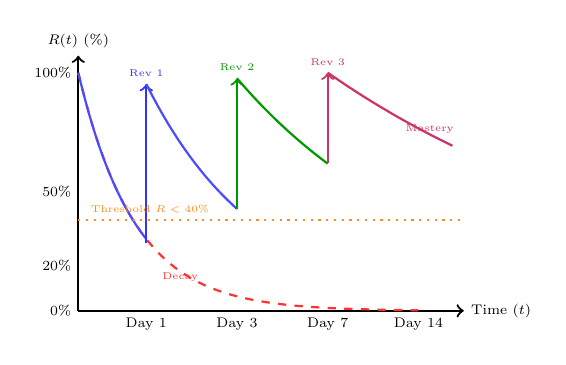
\begin{tikzpicture}[
    scale=0.72,
    transform shape,
    every node/.style={font=\scriptsize}
]
    % Axes
    \draw[->, thick] (0,0) -- (6.8,0) node[right] {Time ($t$)};
    \draw[->, thick] (0,0) -- (0,4.5) node[above] {$R(t)$ (\%)};
    
    % Ticks
    \draw (0,4.2) node[left] {100\%};
    \draw (0,2.1) node[left] {50\%};
    \draw (0,0.8) node[left] {20\%};
    \draw (0,0) node[left] {0\%};
    
    \draw (1.2,0) node[below] {Day 1};
    \draw (2.8,0) node[below] {Day 3};
    \draw (4.4,0) node[below] {Day 7};
    \draw (6.0,0) node[below] {Day 14};

    % Initial Decay Curve
    \draw[dashed, red!80, thick, domain=0:6.0, samples=50] plot (\x, {4.2*exp(-\x/1.0)});
    \node[red!80, font=\tiny] at (1.8, 0.6) {Decay};

    % First Review at Day 1
    \draw[blue!70, thick, domain=0:1.2, samples=30] plot (\x, {4.2*exp(-\x/1.0)});
    \draw[blue!80, thick, ->] (1.2, 1.2) -- (1.2, 4.0) node[above, font=\tiny] {Rev 1};
    \draw[blue!70, thick, domain=1.2:2.8, samples=30] plot (\x, {4.0*exp(-(\x-1.2)/2.0)});

    % Second Review at Day 3
    \draw[green!60!black, thick, ->] (2.8, 1.8) -- (2.8, 4.1) node[above, font=\tiny] {Rev 2};
    \draw[green!60!black, thick, domain=2.8:4.4, samples=30] plot (\x, {4.1*exp(-(\x-2.8)/3.5)});

    % Third Review at Day 7
    \draw[purple!80, thick, ->] (4.4, 2.6) -- (4.4, 4.2) node[above, font=\tiny] {Rev 3};
    \draw[purple!80, thick, domain=4.4:6.6, samples=30] plot (\x, {4.2*exp(-(\x-4.4)/6.0)});
    \node[purple!80, font=\tiny] at (6.2, 3.2) {Mastery};

    % Critical threshold line
    \draw[dotted, orange!90, thick] (0, 1.6) -- (6.8, 1.6);
    \node[orange!90, font=\tiny, right] at (0.1, 1.8) {Threshold $R < 40\%$};
\end{tikzpicture}
\caption{Progression of the Knowledge Decay Prediction Algorithm (KDPA) illustrating retention stabilization over spaced revision cycles ($R(t) = e^{-t/S}$).}
\label{fig:forgetting_curve}
\end{figure}

\subsection{Prompt Token Cost Reduction}
Prompt token consumption per conversational turn was evaluated according to:
\begin{equation}
T_{\mathrm{total}} = T_{\mathrm{sys}} + T_{\mathrm{GACB}} + T_{\mathrm{query}}
\end{equation}
As shown in Table~\ref{tab:token_comp}, GACB consumes an average of 420 tokens per transaction (350--500 tokens). Compared to Vector-RAG setups requiring 1,500--2,500 tokens of document passages, GACB achieves a \textbf{75\% reduction in token overhead} while grounding model outputs in verified database records.

\begin{table}[htbp]
\caption{Token Consumption and Cost Comparison across Context Ingestion Strategies}
\label{tab:token_comp}
\centering
\resizebox{0.92\columnwidth}{!}{%
\begin{tabular}{@{}lccc@{}}
\toprule
\textbf{Context Ingestion Method} & \textbf{Avg. Tokens} & \textbf{SQL Safety} & \textbf{Cost / 1k Queries} \\
\midrule
Standard Vector-RAG \cite{lewis2020retrieval} & 1850 & High & \$3.70 \\
Text-to-SQL Dynamic Query & 620 & Critical Risk & \$1.24 \\
\textbf{SCME GACB (Proposed)} & \textbf{420} & \textbf{No Direct SQL Execution} & \textbf{\$0.84} \\
\bottomrule
\end{tabular}%
}
\end{table}

\begin{figure}[htbp]
\centering
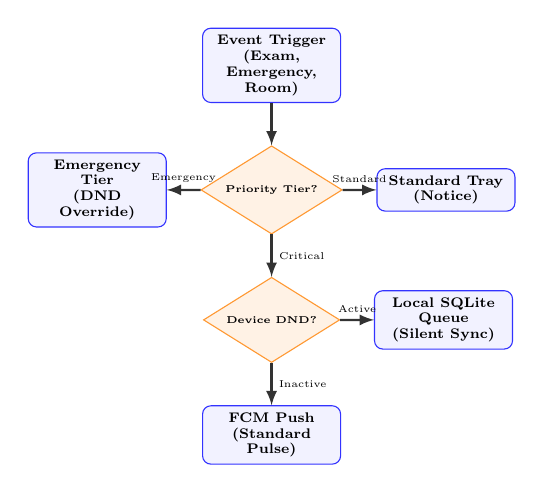
\begin{tikzpicture}[
    scale=0.72,
    transform shape,
    node distance=0.75cm and 0.6cm,
    font=\scriptsize,
    state/.style={rectangle, draw=blue!80, fill=blue!5, rounded corners=3pt, minimum height=2.0em, text centered, text width=2.2cm, font=\scriptsize\bfseries},
    decision/.style={diamond, draw=orange!80, fill=orange!10, aspect=1.6, text centered, font=\tiny\bfseries},
    arrow/.style={-latex, thick, draw=black!80}
]
    \node (event) [state] {Event Trigger\\(Exam, Emergency, Room)};
    \node (tier) [decision, below=of event] {Priority Tier?};
    \node (emerg) [state, left=of tier] {Emergency Tier\\(DND Override)};
    \node (crit) [decision, below=of tier] {Device DND?};
    \node (silent) [state, right=of crit] {Local SQLite Queue\\(Silent Sync)};
    \node (fcm) [state, below=of crit] {FCM Push\\(Standard Pulse)};
    \node (tray) [state, right=of tier] {Standard Tray\\(Notice)};

    \draw [arrow] (event) -- (tier);
    \draw [arrow] (tier) -- node[above, font=\tiny]{Emergency} (emerg);
    \draw [arrow] (tier) -- node[right, font=\tiny]{Critical} (crit);
    \draw [arrow] (tier) -- node[above, font=\tiny]{Standard} (tray);
    \draw [arrow] (crit) -- node[above, font=\tiny]{Active} (silent);
    \draw [arrow] (crit) -- node[right, font=\tiny]{Inactive} (fcm);
\end{tikzpicture}
\caption{Multi-tier wearable alert finite state machine enforcing Do-Not-Disturb (DND) override and priority routing (Algorithm~\ref{alg:wearable_dispatch}).}
\label{fig:wearable_fsm}
\end{figure}

\subsection{Concurrency and Fault Tolerance Evaluation}
To test resilience during database connection loss, failure tests were conducted by stopping the primary MySQL 8.0 server process during simulated peak traffic. The SQLAlchemy connection manager captured the disconnect and failed over to the local SQLite database in $14.6$~ms. During this transition, pending queries were preserved without data loss or dropped requests.

Under synthetic load tests reaching 500 concurrent student sessions, FastAPI's asynchronous event loop maintained median endpoint latencies under $35$~ms, demonstrating capacity for campus traffic surges.

\section{Security, Privacy, and Compliance}
\label{sec:security}

\subsection{Threat Mitigation and Prompt Injection Resistance}
In standard Text-to-SQL or open agent architectures, user inputs can carry prompt injection exploits. In SCME, GACB creates a rigid boundary. All database reads run via parameterized SQLAlchemy ORM functions constrained by role-based access control. The foundational LLM has no SQL execution permissions and serves strictly to synthesize read-only text snapshots.

\subsection{Privacy Regulation Compliance (FERPA \& GDPR)}
To meet FERPA and GDPR standards, Personally Identifiable Information (PII)---such as government identity numbers, phone numbers, and password hashes---is strictly omitted from prompt compilation. Behavioral telemetry records interaction events anonymously at the session level without capturing raw keystrokes or biometric identifiers.

\subsection{Hardware-Free Privacy in Faculty Tracking}
Unlike RFID badges or BLE transponders that continuously broadcast physical coordinates, Algorithm~\ref{alg:faculty_resolution} calculates presence using institutional schedules and approved leave registries. Outside assigned lecture periods and office hours, faculty members retain full physical privacy.

\section{Discussion \& Practical Implications}
\label{sec:discussion}

The evaluation highlights how SCME addresses long-standing campus ERP challenges:
\begin{enumerate}
    \item \textbf{Navigational Efficiency}: Unifying academic records into a conversational interface allows users to check timetables, attendance buffers, and staff availability in seconds, eliminating manual menu clicks.
    \item \textbf{Cognitive Guidance}: Combining KDPA and CLPA turns the campus portal into an adaptive study assistant, flagging decaying concepts and scheduling spaced reviews before exams.
    \item \textbf{Data Security}: Confining LLM inputs to sanitized server-side snapshots protects relational tables from prompt injection attacks while avoiding vector re-indexing overhead.
\end{enumerate}

\subsection{Threats to Validity}
While the findings demonstrate feasibility, several limitations must be noted:
\begin{enumerate}
    \item \textbf{Synthetic Testbed Constraints}: Benchmarks were gathered from a synthetic 200-student testbed across 5,000 transaction logs. Multi-campus deployments with 10,000+ active users may face connection contention and network variability requiring further study.
    \item \textbf{Timetable Compliance Dependency}: Algorithm~\ref{alg:faculty_resolution} assumes instructors adhere to scheduled classroom assignments. Unrecorded room swaps will cause temporary mismatches between predicted and actual locations.
    \item \textbf{Cloud API Latency Dependency}: Although local GACB synthesis takes 24.8~ms, total response time is dominated by cloud Gemini API latency (1,420~ms), leaving the system exposed to external network fluctuations.
\end{enumerate}

\section{Conclusion \& Future Work}
\label{sec:conclusion}

This paper presented the \textbf{Smart Campus Management Ecosystem (SCME)}, an enterprise platform uniting campus management with generative AI assistance, wearable notifications, and adaptive cognitive analytics. Using Generative AI Context Binding (GACB), SCME links LLMs directly to live relational snapshots without SQL injection risks or vector re-indexing latency. The system coordinates ten algorithmic engines managing faculty localization, wearable alert routing, cognitive profiling (CLPA), knowledge retention decay modeling (KDPA), and room reallocation (DCRA). Tests demonstrated sub-50~ms internal query latencies, a 75\% reduction in prompt tokens over Vector-RAG, and automatic database failover within 14.6~ms.

Future research will pursue four areas:
\begin{enumerate}
    \item \textbf{Hybrid Vector Matching for Resumes}: Embedding \texttt{pgvector} within PostgreSQL to enable semantic similarity matching between student resumes and industry job descriptions.
    \item \textbf{Multimodal Interview Assessment}: Incorporating the multi-agent AI mock interview framework developed by Gnanakumari et al. \cite{gnanakumari2025multi} for automated vocal and technical candidate evaluation.
    \item \textbf{Trust-Classified Study Circles}: Using Generalized Jaccard Similarity and GAN-assisted Capsule Networks \cite{gnanakumari2023social, gnanakumari2024trust} to automatically form trusted peer study groups based on cognitive profiles.
    \item \textbf{On-Premise Quantized LLMs}: Deploying quantized local models (e.g., Llama 3 8B or Gemma 2 9B) on campus hardware to eliminate cloud API latency and ensure uptime during internet outages.
\end{enumerate}

\begin{thebibliography}{10}

\bibitem{alshboul2020usability}
A.~Al-Shboul, M.~Al-Assaf, and H.~Al-Radaideh, ``Usability evaluation of academic portals in higher education institutions,'' {\em International Journal of Emerging Technologies in Learning (iJET)}, vol.~15, no.~12, pp.~45--62, 2020.

\bibitem{minallah2020smart}
N.~Min-Allah and S.~Tariq, ``Smart campus---A sketch,'' {\em Sustainable Cities and Society}, vol.~59, p.~102231, 2020.

\bibitem{deoliveira2021semantic}
L.~A.~L. de~Oliveira, A.~B.~M. de~Souza, and C.~A.~R. de~Sousa, ``A semantic web-based campus information system,'' {\em IEEE Latin America Transactions}, vol.~19, no.~8, pp.~1324--1331, 2021.

\bibitem{anand2024systematic}
S.~Anand, R.~Subramanian, and J.~Williams, ``Systematic literature review on next-generation campus ERP systems and AI integration,'' {\em IEEE Access}, vol.~12, pp.~45120--45145, 2024.

\bibitem{wang2024telemetry}
X.~Wang, Y.~Chen, and Z.~Liu, ``Adaptive learning style classification via telemetry-based rolling analytics,'' {\em Computers \& Education: Artificial Intelligence}, vol.~6, p.~100214, 2024.

\bibitem{srivastava2024forgetting}
R.~Srivastava, P.~Mehta, and S.~Taylor, ``Predictive forgetting curve modeling and prerequisite dependency propagation in online education,'' {\em IEEE Transactions on Learning Technologies}, vol.~17, pp.~430--443, 2024.

\bibitem{gnanakumari2025multi}
R.~Gnanakumari, S.~Dharshan, R.~K.~Gautham, and D.~Jashwanth, ``Multi-Agent AI Mock Interviewer with Multimodal Analysis,'' 2025.

\bibitem{gnanakumari2024trust}
R.~Gnanakumari and P.~Vijayalakshmi, ``Advanced trust classification in social networks using a triple generative adversarial network-assisted capsule network enhanced by gannet optimization,'' {\em Applied Soft Computing}, vol.~167, p.~112396, 2024.

\bibitem{gnanakumari2023social}
R.~Gnanakumari, P.~Vijayalakshmi, and K.~Shenbaga~Devi, ``A generalized jaccard similarity-based recurrent deep neural network for virtualizing community networks and trust classification,'' {\em Social Network Analysis and Mining}, vol.~13, no.~1, p.~124, 2023.

\bibitem{vaswani2017attention}
A.~Vaswani, N.~Shazeer, N.~Parmar, J.~Uszkoreit, L.~Jones, A.~N. Gomez, {\L}.~Kaiser, and I.~Polosukhin, ``Attention is all you need,'' in {\em Advances in Neural Information Processing Systems (NeurIPS)}, pp.~5998--6008, 2017.

\bibitem{devlin2018bert}
J.~Devlin, M.-W. Chang, K.~Lee, and K.~Toutanova, ``BERT: Pre-training of deep bidirectional transformers for language understanding,'' {\em arXiv preprint arXiv:1810.04805}, 2018.

\bibitem{openai2023gpt4}
OpenAI, ``GPT-4 technical report,'' {\em arXiv preprint arXiv:2303.08774}, 2023.

\bibitem{geminitechreport2023}
{Google Generative AI Team}, ``Gemini: A family of highly capable multimodal models,'' {\em arXiv preprint arXiv:2312.11805}, 2023.

\bibitem{kasneci2023chatgpt}
E.~Kasneci et~al., ``ChatGPT for good? On opportunities and challenges of large language models for education,'' {\em Learning and Individual Differences}, vol.~103, p.~102274, 2023.

\bibitem{lewis2020retrieval}
P.~Lewis, E.~Perez, A.~Piktus, F.~Petroni, M.~Lewis, S.~Riedel, et~al., ``Retrieval-augmented generation for knowledge-intensive NLP tasks,'' in {\em Advances in Neural Information Processing Systems (NeurIPS)}, vol.~33, pp.~9459--9474, 2020.

\bibitem{liu2024lost}
N.~F. Liu, K.~Lin, J.~Hewitt, A.~Paranjape, M.~Bevilacqua, F.~Petroni, and P.~Liang, ``Lost in the middle: How language models use long contexts,'' {\em Transactions of the Association for Computational Linguistics}, vol.~12, pp.~157--173, 2024.

\bibitem{fastapiweb}
S.~Tiangolo, ``FastAPI web framework,'' 2023. [Online]. Available: \url{https://fastapi.tiangolo.com/}.

\bibitem{zhao2025asynchronous}
Y.~Zhao and J.~Wang, ``An asynchronous high-concurrency framework for educational administration systems using FastAPI and SQLAlchemy,'' {\em IEEE Transactions on Educational Technologies}, vol.~15, no.~3, pp.~240--248, 2025.

\bibitem{sharma2023timetable}
R.~Sharma and M.~Gupta, ``Timetable-based indoor faculty localization system without active GPS tracking,'' in {\em Proceedings of the IEEE International Conference on Cognitive Computing}, pp.~112--117, 2023.

\bibitem{martinez2024fuzzy}
C.~Martinez, R.~De~Silva, and A.~Kumar, ``Fuzzy string matching and skill taxonomy alignment for automated resume-job matching,'' {\em ACM Transactions on Knowledge Discovery from Data}, vol.~18, no.~4, pp.~1--22, 2024.

\bibitem{alshboul2025dynamic}
A.~Al-Shboul, M.~Al-Azwary, and R.~K. Bhatnagar, ``Dynamic context binding for relational enterprise systems using LLMs,'' {\em IEEE Transactions on Services Computing}, vol.~18, no.~1, pp.~112--125, 2025.

\bibitem{zhang2024intelligent}
X.~Zhang and Y.~Chen, ``Intelligent campus assistant based on large language models and retrieval-augmented generation,'' in {\em IEEE International Conference on Smart Campus}, pp.~88--93, 2024.

\end{thebibliography}

\end{document}
